\documentclass[tikz,border=3pt]{standalone}
\usepackage[utf8]{inputenc}
\usepackage[T1]{fontenc}
\usepackage{libertinus}
\usepackage{amsmath,amssymb}
\usetikzlibrary{arrows.meta,calc,patterns,decorations.pathmorphing,decorations.markings,decorations.pathreplacing,bending}
\definecolor{UGblue}{RGB}{0,51,102}
\newcommand{\dbar}{\mathchar'26\mkern-12mu d}
\tikzset{
  >=Stealth,
  every node/.style={font=\small},
  caja/.style={draw,line width=0.9pt},
  pared/.style={draw,line width=1.6pt},
  ejes/.style={->,line width=0.8pt},
  adia/.style={draw,pattern=north east lines,pattern color=black!70,line width=0.5pt},
  gas/.style={fill=UGblue!8},
  punto/.style={fill,circle,inner sep=1.3pt},
  onda/.style={decorate,decoration={snake,amplitude=1.1pt,segment length=5pt,post length=3pt,pre length=0pt}},
}
\begin{document}
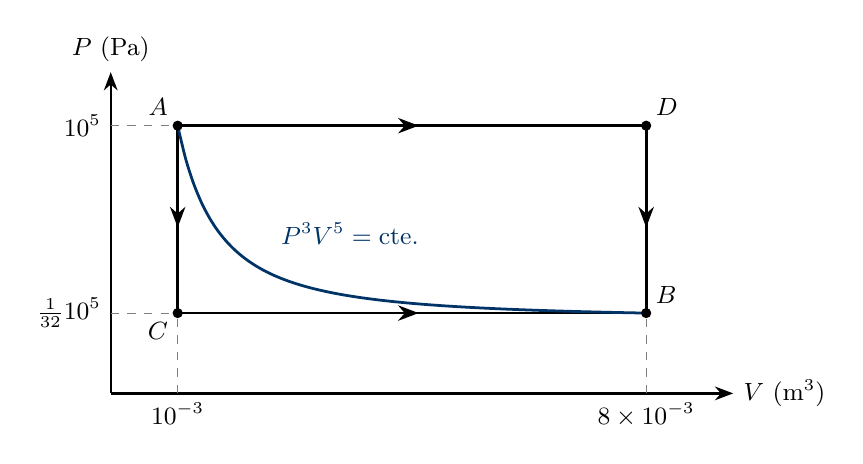
\begin{tikzpicture}[xscale=0.85,yscale=3.4]
  \draw[ejes] (0,0) -- (9.3,0) node[right] {$V\ (\mathrm{m^3})$};
  \draw[ejes] (0,0) -- (0,1.2) node[above] {$P\ (\mathrm{Pa})$};
  \draw[dashed,gray,line width=0.4pt] (0,1) -- (1,1); \draw[dashed,gray,line width=0.4pt] (0,0.3) -- (1,0.3);
  \draw[dashed,gray,line width=0.4pt] (1,0) -- (1,1); \draw[dashed,gray,line width=0.4pt] (8,0) -- (8,1);
  \node[left] at (0,1) {$10^{5}$};
  \node[left] at (0,0.3) {$\tfrac{1}{32}10^{5}$};
  \node[below] at (1,0) {$10^{-3}$};
  \node[below] at (8,0) {$8\times10^{-3}$};
  \draw[line width=1pt,-{Stealth[length=2.6mm]}] (1,1) -- (4.6,1);
  \draw[line width=1pt] (4.5,1) -- (8,1);
  \draw[line width=1pt,-{Stealth[length=2.6mm]}] (8,1) -- (8,0.62);
  \draw[line width=1pt] (8,0.65) -- (8,0.3);
  \draw[line width=1pt,-{Stealth[length=2.6mm]}] (1,1) -- (1,0.62);
  \draw[line width=1pt] (1,0.65) -- (1,0.3);
  \draw[line width=1pt,-{Stealth[length=2.6mm]}] (1,0.3) -- (4.6,0.3);
  \draw[line width=1pt] (4.5,0.3) -- (8,0.3);
  \draw[line width=1pt,UGblue,domain=1:8,samples=60,smooth,variable=\x] plot ({\x},{0.3+0.7*(exp(-5/3*ln(\x))-1/32)/(31/32)});
  \node[punto] at (1,1) {}; \node[punto] at (8,1) {}; \node[punto] at (1,0.3) {}; \node[punto] at (8,0.3) {};
  \node[above left] at (1,1) {$A$}; \node[above right] at (8,1) {$D$};
  \node[below left] at (1,0.3) {$C$}; \node[above right] at (8,0.3) {$B$};
  \node[UGblue,above right] at (2.4,0.52) {$P^{3}V^{5}=\text{cte.}$};
\end{tikzpicture}
\end{document}
